%---------
% place your email id between the braces so that your homework has a name
\def\yourname{Mark Xiong}
% -----------------------------------------------------
\def\duedate{4/19/24}
\def\duelocation{via \href{https://www.gradescope.com/courses/753885}{Gradescope}}
\def\hnumber{5}
\def\prof{Lorenzo Orecchia}
\def\course{\href{https://canvas.uchicago.edu/courses/56880}{CMSC 27200 - Spring 2024}}
%-------------------------------------

\documentclass[10pt]{article}
\usepackage[colorlinks,urlcolor=blue]{hyperref}
\usepackage[osf]{mathpazo}
\usepackage{amsmath,amsfonts,graphicx}
\usepackage{latexsym}
%\usepackage{subfig}
\usepackage{algpseudocode}
\usepackage[shortlabels]{enumitem}
\usepackage{algorithm}
\usepackage{listings}

\usepackage{tkz-graph}
\usepackage{tikz}
\usetikzlibrary{arrows.meta,arrows}
\usepackage{qtree}
\usepackage{tikz-qtree}
\usepackage{subcaption}
\usepackage{float}   

%\usepackage[top=1in,bottom=1.4in,left=1.5in,right=1.5in,centering]{geometry}
\usepackage{fullpage}
\usepackage{color}
\definecolor{mdb}{rgb}{0.3,0.02,0.02} 
\definecolor{cit}{rgb}{0.05,0.2,0.45}
\usepackage{wrapfig}
%\pagestyle{myheadings}
\markboth{Haoxiang}{\yourname}

\thispagestyle{empty}

\newenvironment{proof}{\par\noindent{\it Proof.}\hspace*{1em}}{$\Box$\bigskip}
\newcommand{\qed}{$\Box$}
\newcommand{\alg}[1]{\mathsf{#1}}
\newcommand{\handout}{
   \renewcommand{\thepage}{H\hnumber-\arabic{page}}
   \noindent
   \begin{center}
      \vbox{
    \hbox to \columnwidth {\sc{\course} --- \prof \hfill}
    \vspace{-2mm}
    \hbox to \columnwidth {\sc due \MakeLowercase{\duedate} \duelocation\hfill {\Huge\color{mdb}H\hnumber.\yourname}}
      }
   \end{center}
   \vspace*{2mm}
}
\newcommand{\solution}[1]{
\vspace{2mm}

\noindent Collaborators:

\vspace{5mm}

\medskip\noindent{\color{cit}\textbf{Solution:} #1}}

\newcommand{\bit}[1]{\{0,1\}^{ #1 }}
\newcommand{\extraspace}{\medskip\noindent{\color{cit} Extra space for your solution}\newpage}
%\dontprintsemicolon
%\linesnumbered=
\newtheorem{problem}{\sc\color{cit}Problem}
\newtheorem{lemma}{Lemma}
\newtheorem{theorem}{Theorem}
\newtheorem{definition}{Definition}
\newtheorem{claim}{Claim}


\begin{document}
\handout
\begin{itemize}
\item The assignment is due at Gradescope on \duedate.

\item A LaTeX template will be provided for each homework. You are strongly encouraged to type your homework into this template using \LaTeX.  If you are writing by hand, please fill in the solutions in this template, inserting additional sheets as necessary. This will help facilitate the grading.

\item You are permitted to discuss the problems with up to 2 other students in the class (per problem); however, {\em you must write up your own solutions, in your own words}. Do not submit anything you cannot explain. If you do collaborate with any of the other students on any problem, please list all your collaborators in the appropriate spaces.

\item Similarly, please list any other source you have used for each problem, including other textbooks or websites.

\item {\em Show your work.} Answers without justification will be given little credit.

\item Your homework is \textit{resubmittable}. Please refer to the course syllabus on Canvas for a more detailed description of this. For any problem that you have not changed from your last submission, please make sure to indicate this in your submission to help our graders grade faster. 

\item Is anyone still reading these?

\end{itemize}

%%%%%%%%%%%%%%%%%%%%%%%%%%%%%%%%%%%%%%%%%%%
% QUESTION 1
%%%%%%%%%%%%%%%%%%%%%%%%%%%%%%%%%%%%%%%%%%%

\newpage
\begin{problem}[Midterm True / False] 
For the following statements, state whether the statement is true or false. If the answer is true, provide a brief explanation why; if the answer is false, provide a counter example.
\begin{enumerate}[(a)]
\item For any pair of functions $f(n), g(n)$, if $f(n) = O\big( g(n) \big)$, then $\log\big( f(n) \big) = O\big( \log ( g(n)) \big)$.

\item For any pair of functions $f(n), g(n)$, if $f(n) = \Omega\big( g(n) \big)$, then $\log\big( f(n) \big) = \Omega\big( \log( g(n)) \big)$.

\item Let $\mathcal{A}$ be a divide-and-conquer algorithm which takes an input of size $n$, and recursively calls itself. In a single call, it recursively calls itself 8 times, on inputs of size $n / 2$. Suppose the work done outside of the recursion (i.e. the merging step) takes time $O(n^d)$ for some constant $d$. For any $d \geq 2$, the running time of the algorithm can be then be bounded by $O\big( n^d \big)$.

\item Every fourth root of unity is also an eighth root of unit.

\item Every DAG has at least one source and one sink vertex.

\item Every directed graph with at least one source, and one sink will be a DAG.

\item Given any graph $G = (V, E)$ with edge weights $w_e$, Dijkstra's algorithm can be used to find the shortest path between any two vertices $s, t \in V$, even if $G$ has negative weight.
\end{enumerate}
    
\end{problem}

\begin{solution}
    The solution is as follows:
    \begin{enumerate} [(a)]
        \item False. Consider $f(n) = 1, g(n) = 2: \log(f(n)) = 0$ and $\log(g(n)) = O(1)$.
        \item \textcolor{blue}{False. Consider $f(n) = 1, g(n) = 2: f(n) = \Omega(g(n))$, but we have $\log(f(n)) = 0$ and $\log(g(n)) = O(1)$.}
        \item False. $T(n) = 8T(n/2) + O(n^d)$ is $O(n^d)$ for $d > 3$. Applying Master Theorem gives that it's false for $d < 3$. When $d = 2$, we have $O(n^{\log_b a})$ = $O(n^{\log_2 8}) = O(n^3)$.
        \item True. Fourth roots of unity are $1, -1, i, -i$. When they are raised to the eighth power, they also yield 1. So, every fourth root of unity is also an eighth root of unity.
        \item True. Start with any vertex $v$, Since there are no cycles, you cannot keep moving backwards indefinitely. If you attempt to move backwards from 
        v to its predecessors repeatedly, because there are no cycles, you must eventually reach a vertex that has no predecessors. Similarly, you cannot continue the process of finding successors indefinitely, therefore you must eventually reach a vertex that has no successors, which is a sink.
        \item False. Consider a graph with a line-like structure, with a source at one end and a sink at the other. If you add an edge from the a node in the middle to another node in the middle before it, the graph will no longer be a DAG as it forms a cycle.
        \item False. Consider an triangle with nodes A B C, with edge weights AB = 3, BC = -2, AC = 2. Dijkstra's algorithm will return a shortest path from A to C as A -> C, with a total weight of 2. However, the shortest path is A -> B -> C with a total weight of 1.
    \end{enumerate}   
\end{solution}

%%%%%%%%%%%%%%%%%%%%%%%%%%%%%%%%%%%%%%%%%%%
% QUESTION 2
%%%%%%%%%%%%%%%%%%%%%%%%%%%%%%%%%%%%%%%%%%%


\newpage
\begin{problem}
    Show the running of Dijkstra's algorithm for finding the shortest distance from $A$ to all other vertices in the graph from Figure~\ref{fig:dijkstra-directed}. You should show the updated distance estimates to all the vertices (i.e., the key of the vertex in the priority queue) after each time a vertex is extracted from the priority queue in the algorithm. (Fill in the following table with the distances from $A$ to all other vertices. Each row represents the distances after one more vertex is removed from the queue.)

    \begin{figure}[h]
        \centering
        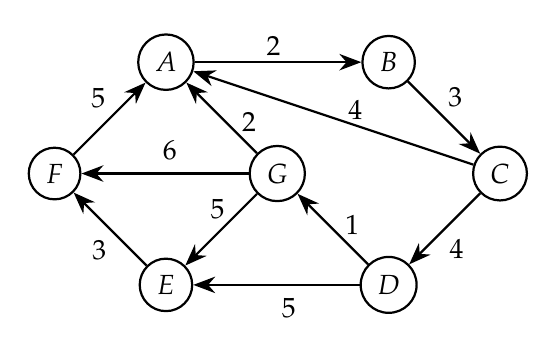
\begin{tikzpicture}[node distance={20mm}, thick,main/.style={circle, thick,draw,font=\sffamily\bfseries}, ar/.style={-{Stealth[scale=1.2]}}]
          \node[main] (1) {$G$};
          \node[main] (2) [above left of=1]{$A$};
          \node[main] (3) [above right of=1]{$B$};
          \node[main] (4) [below right of=3]{$C$};
          \node[main] (5) [below left of=4]{$D$};
          \node[main] (6) [below left of=1]{$E$};
          \node[main] (7) [below left of=2]{$F$};
          
          \draw[ar] (1) -- (2) node [at start, xshift=-0.1cm, yshift=0.4cm]{$2$};
          \draw[ar] (1) -- (6) node [at start, xshift=-0.5cm, yshift=-0.2cm]{$5$};
          \draw[ar] (1) -- (7) node [at start, xshift=-1.0cm, yshift=0.3cm]{$6$};
          \draw[ar] (2) -- (3) node [at start, xshift=1.0cm, yshift=0.2cm]{$2$};
          \draw[ar] (3) -- (4) node [at start, xshift=0.6cm, yshift=-0.2cm]{$3$};
          \draw[ar] (4) -- (2) node [at start, xshift=-1.5cm, yshift=0.7cm]{$4$};
          \draw[ar] (4) -- (5) node [at end, xshift=0.6cm, yshift=0.2cm]{$4$};
          \draw[ar] (5) -- (1) node [at start, xshift=-0.2cm, yshift=0.5cm]{$1$};
          \draw[ar] (5) -- (6) node [at start, xshift=-0.9cm, yshift=-0.3cm]{$5$};
          \draw[ar] (6) -- (7) node [at start, xshift=-0.6cm, yshift=0.2cm]{$3$};;
          \draw[ar] (7) -- (2) node [at end, xshift=-0.6cm, yshift=-0.2cm]{$5$};;
        \end{tikzpicture}
        \caption{A directed weighted graph $G$.}
        \label{fig:dijkstra-directed}
    \end{figure}

        
    \begin{center}
    \begin{tabular}{|c|c|c|c|c|c|c|c|}
    \hline
         Key in Queue: & A & B & C & D & E & F & G\\
         \hline 
         Step 1: -& \;\text{ $0$ }\; & \;$\infty$\; & \;$\infty$\; & \;$\infty$\; & \;$\infty$\; & \;$\infty$\; & \;$\infty$\;\\
         \hline
         Step 2: & \;\text{ $0$ }\; & 2 & \;$\infty$\; & \;$\infty$\; & \;$\infty$\; & \;$\infty$\; & \;$\infty$\;\\
         \hline
         Step 3:  & 0 & 2 & 5 & $\infty$ & $\infty$ & $\infty$ & $\infty$\\
         \hline
         Step 4:  & 0 & 2 & 5 & 9 & $\infty$ & $\infty$ & $\infty$\\
         \hline
         Step 5:  & 0 & 2 & 5 & 9 & 14 & $\infty$ & 10 \\
         \hline
         Step 6:  & 0 & 2 & 5 & 9 & 14 & 16 & 10\\
         \hline
         Step 7:  & 0 & 2 & 5 & 9 & 14 & 16 & 10\\
         \hline
         Step 8: & 0 & 2 & 5 & 9 & 14 & 16 & 10\\
         \hline

    \end{tabular}
\end{center}
\end{problem}

\end{document}
